%%%%%%%%%%%%%%%%%%%%%%%%%%%%%%%%%%%%%%%%%%%%%%%%%%%%%%%%%%%
% EPFL report package, main thesis file
% Goal: provide formatting for theses and project reports
% Author: Mathias Payer <mathias.payer@epfl.ch>
%
% To avoid any implication, this template is released into the
% public domain / CC0, whatever is most convenient for the author
% using this template.
%
%%%%%%%%%%%%%%%%%%%%%%%%%%%%%%%%%%%%%%%%%%%%%%%%%%%%%%%%%%%
\documentclass[a4paper,11pt,oneside]{report}
% Options: MScThesis, BScThesis, MScProject, BScProject
\usepackage[MScProject]{EPFLreport}
\usepackage{xspace}

\title{Design and evaluation of mixers\\in a high-churn environment}
\author{Derya Cögendez}
\supervisor{Linus Gasser}
\adviser{Pierluca Borsò-Tan}
%\coadviser{Second Adviser}
\newcommand{\sysname}{FooSystem\xspace}

\begin{document}
\maketitle
\makeacks

\begin{abstract}
Fledger is a peer-to-peer network which works on browsers, it is very modular an can easily be extended with additional services. One of it's services is web proxy which lets peers act as proxies for other nodes. This service can let users their traffic patterns from their ISP, however it does nothing to protect from traffic analysis by an adversary with limited view of the network nor does it hide traffic patterns from the proxy node. In this project, we do literature review to choose a suitable anonymous communication system for this specific use case of web proxy. We create a proof of concept implementation and fine tune and evaluate it in the setting of Fledger. 


\textbf{Given Fledger is a peer to peer network and churn is inevitable, we then add simple mechanisms to improve the reliability of message delivery in the presence of churn.} 
\textbf{Add the results here}
\end{abstract}

\maketoc

%%%%%%%%%%%%%%%%%%%%%%
\chapter{Introduction}
%%%%%%%%%%%%%%%%%%%%%%
% The introduction is a longer writeup that gently eases the reader into your
% thesis~\cite{dinesh20oakland}. Use the first paragraph to discuss the setting.
% In the second paragraph you can introduce the main challenge that you see.
% The third paragraph lists why related work is insufficient.
% The fourth and fifth paragraphs discuss your approach and why it is needed.
% The sixth paragraph will introduce your thesis statement. Think how you can
% distill the essence of your thesis into a single sentence.
% The seventh paragraph will highlight some of your results
% The eights paragraph discusses your core contribution.

% This section is usually 3-5 pages.
\textbf{Insert something that leads onto fledger without chatgpt speak ( or something about web proxies maybe)}

Fledger\textbf{cite} is a peer-to-peer network designed to work directly in the browser, without the need for proxies. It enables connecting browsers to communicate between nodes. It is under development and will let users share resources like disk space, CPU, and network bandwidth in the future. Fledger's initial use cases are a decentralized chat application and web proxy. Although with the current version of Fledger, one can use the web proxy, there are some privacy concerns with it. \textbf{insert stuff of isp and traffic analysis} Also, the remote node acting as the web proxy can see all the traffic patterns from the user. 

To remedy this issue we first look into different anonymous communications systems. The first anonymous communication system that comes to mind, Tor\textbf{cite}, is vulrable to traffic analysis [cite stuff].
% To our knowledge there isn't much research into using mixnets for web surfing as for a long time mixnetwork have been limited by their high latency.
% Can probably get some inpiration from one of the mixnet papers
Other communications systems such as .... although solves the problem of Tor, they usually have very high latencies unsuitable for an "instantanous" application such as a web proxy.

We choose Loopix Anonymity System \textbf{cite} for it's low latency, apparent scalability (and tunability) and availability of reference implementations.

We integrate Loopix into Fledger, and adapt it for use for the specific purpose of web browsing through a web proxy. We then choose configuration parameters through extensive experimentation. Although the Loopix paper looks extensively into the privacy aspects of the system, they leave reliable message delivery to future work. \textbf{transition} We explore potential ways to improve the reliability of our implementation. Finally we add simple mechanisms to have more reliable message delivery in the presence of churn.

In conclusion:

% Conclusion: integrated loopix anonymity system into fledger and adapted it for the specific purpose of web proxying with low latency and high reliability. 

%%%%%%%%%%%%%%%%%%%%
\chapter{Background}
%%%%%%%%%%%%%%%%%%%%

% The background section introduces the necessary background to understand your
% work. This is not necessarily related work but technologies and dependencies
% that must be resolved to understand your design and implementation.

% This section is usually 3-5 pages.

%-------------------
\section{Fledger}
%-------------------
Fledger is a P2P network run entirely using browsers, it's goal is to enable user to share resources such as CPU, bandwidth, disk space etc. It uses WebRTC to commnunicate and uses a Signaling Server to enable nodes to discover each other.
\textbf{talk about how it can be run through the browser but as a node as well}
%-------------------
\subsection{Communication between nodes}

When a new Fledger node joins the network, it creates a key pair and derives and ID from it. This ID is called a nodeID, it is nodeID is the main routing information for Fledger nodes. 

After the node starts up and creates its routing information, it announces itself to the Signaling server, which in turn gives the node information about other nodes that are online.

When the node wants to communicate with another node, it will send a message to the signaling server. The signaling server will act as a mediator for the two nodes to negotiate a connection. Once the connection is established between the nodes, they can communicate through their browsers.

In \autoref{fig:webrtc}, Peer 1 sends \textit{Signaling} message to the Signaling server to start establishing a connection with Peer 2, they communicate through the signaling server to negotiate the connection. Once the connection is established, they can directly communicate without the need for the Signaling server. 

\begin{figure}[H]
    \centering
    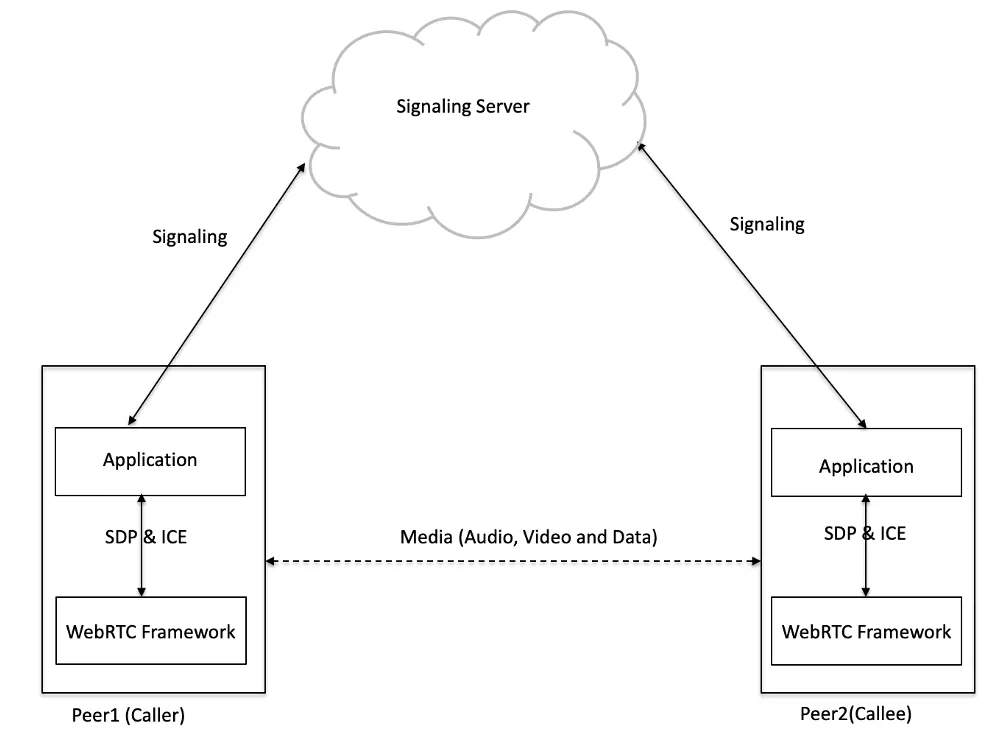
\includegraphics[width=0.8\linewidth]{plots/webrtc.png}
    \caption{}
    \label{fig:webrtc}
    \small\textit{Figure from Medium: "Choice of Signaling Server in Web Real-Time Communication"}
\end{figure}

%-------------------
\subsection{Modules}
\label{sec:fledger_modules}

For each functionality in Fledger, there is a separate module. This section will introduce the relevant Fledger modules to this project.

\begin{itemize}
    \item \textbf{Network} \\
    Network module uses the WebRTC protocol and enables other modules send messages through its messages. It can be used for both browsers and for Fledger nodes. In this project we use Fledger as 
    \item \textbf{Gossip and Random Connections Modules} \\
    Gossiping module enables messages to be propagated through the Fledger network, and it uses Random Connections module. Random Connections module is designed to establish random connections between the nodes, and it uses the network module to send messages to the selected nodes. These two module are used for the bootstrapping of the Loopix Module for the purpose of experimentation. See \textbf{autoref} for further details about the bootstrapping.
    \item \textbf{Web Proxy} \\
    Web proxy module handles web proxy requests, it can be used to create and respond to request to get web pages. It creates a unique ID for a request and sends the message. When a node responds to a request, it sends multiple messages with the same unique ID as the request, which enables the web proxy client to collect the messages into the requested page. If the client does not receive the complete response within a set period of time, the request will timeout.
    \item \textbf{Overlay} \\
    This module acts as a translator/wrapper for Fledger modules. While sending a message through gossip or web proxy this module will wrap the message and then send it to the specific module. For example if node A wants to send a web proxy message to node B, node A will create web proxy message, which will be sent to Overlay module, still within node A, and Overlay module will translate for the corresponding module, for example random connections, and send the translated message to this module, which will finally send the message to the network module, and the message will be sent to node B through the WebRTC connection. Linus Gasser has kindly created this module to help integrate Loopix module into Fledger.
    \item \textbf{Loopix} \\
    In this project we have created a Loopix module that can be used as a middle man between any module and the network module. The main purpose is to be used with web proxy but it can be used to send other kinds of messages from Fledger modules as long as they are sent through an Overlay. See the next section \textbf{autoref} for more detailed information about the Loopix Anonymity System. 
\end{itemize}

%-------------------
\section{The Loopix Anonymity System}
%-------------------
Loopix is a continuous time mix network. Unlike the traditional mix networks introduced by \textbf{cite chaum here}, in continuous time mix networks, which operate in rounds. Packets are stopped for a time at the mix node and then sent on their ways. This delay is usually drawn from an exponential dsitribution \textbf{cite}.

Loopix combines this stop-and-go \textbf{maybe i need to cite the paper that called it that?} mixing with cover traffic to further hide traffic patterns and avoid \textbf{find attacks (n-1?) , which were possible with  networks.}

Quite like the Tor network, the route of the message is chosen by the client in advance and the messages are encapsulated in layers of encryption with public keys each of the nodes in the route. However, unlike the Tor network, each message goes through a separate route, with a different delay at each hop of the route. \textbf{talk about how this makes it harder to do traffic analysis}.

There are three different roles in the Loopix network. Nodes which use the mix network are called \textit{clients}. Clients have \textit{providers}, providers act as entry nodes to the network for the clients. A client sends all their traffic through their provider. In turn, the provider forwards the clients messages to the mix network and stores message, in which the final destination is the client. If the client is online, it will ask the provider for the messages it is storing.

Finally, there are mix nodes. Mix nodes are arranged in a stratified topology \textbf{cite}, and their main purpose is to \textit{unwrap} messages that they receive, wait for the delay specified in the header of the unwrapped packet, and then send the message to the next hop. The mix node only knows about the delay, and previous and next nodes.

\begin{figure}[H]
    \centering
    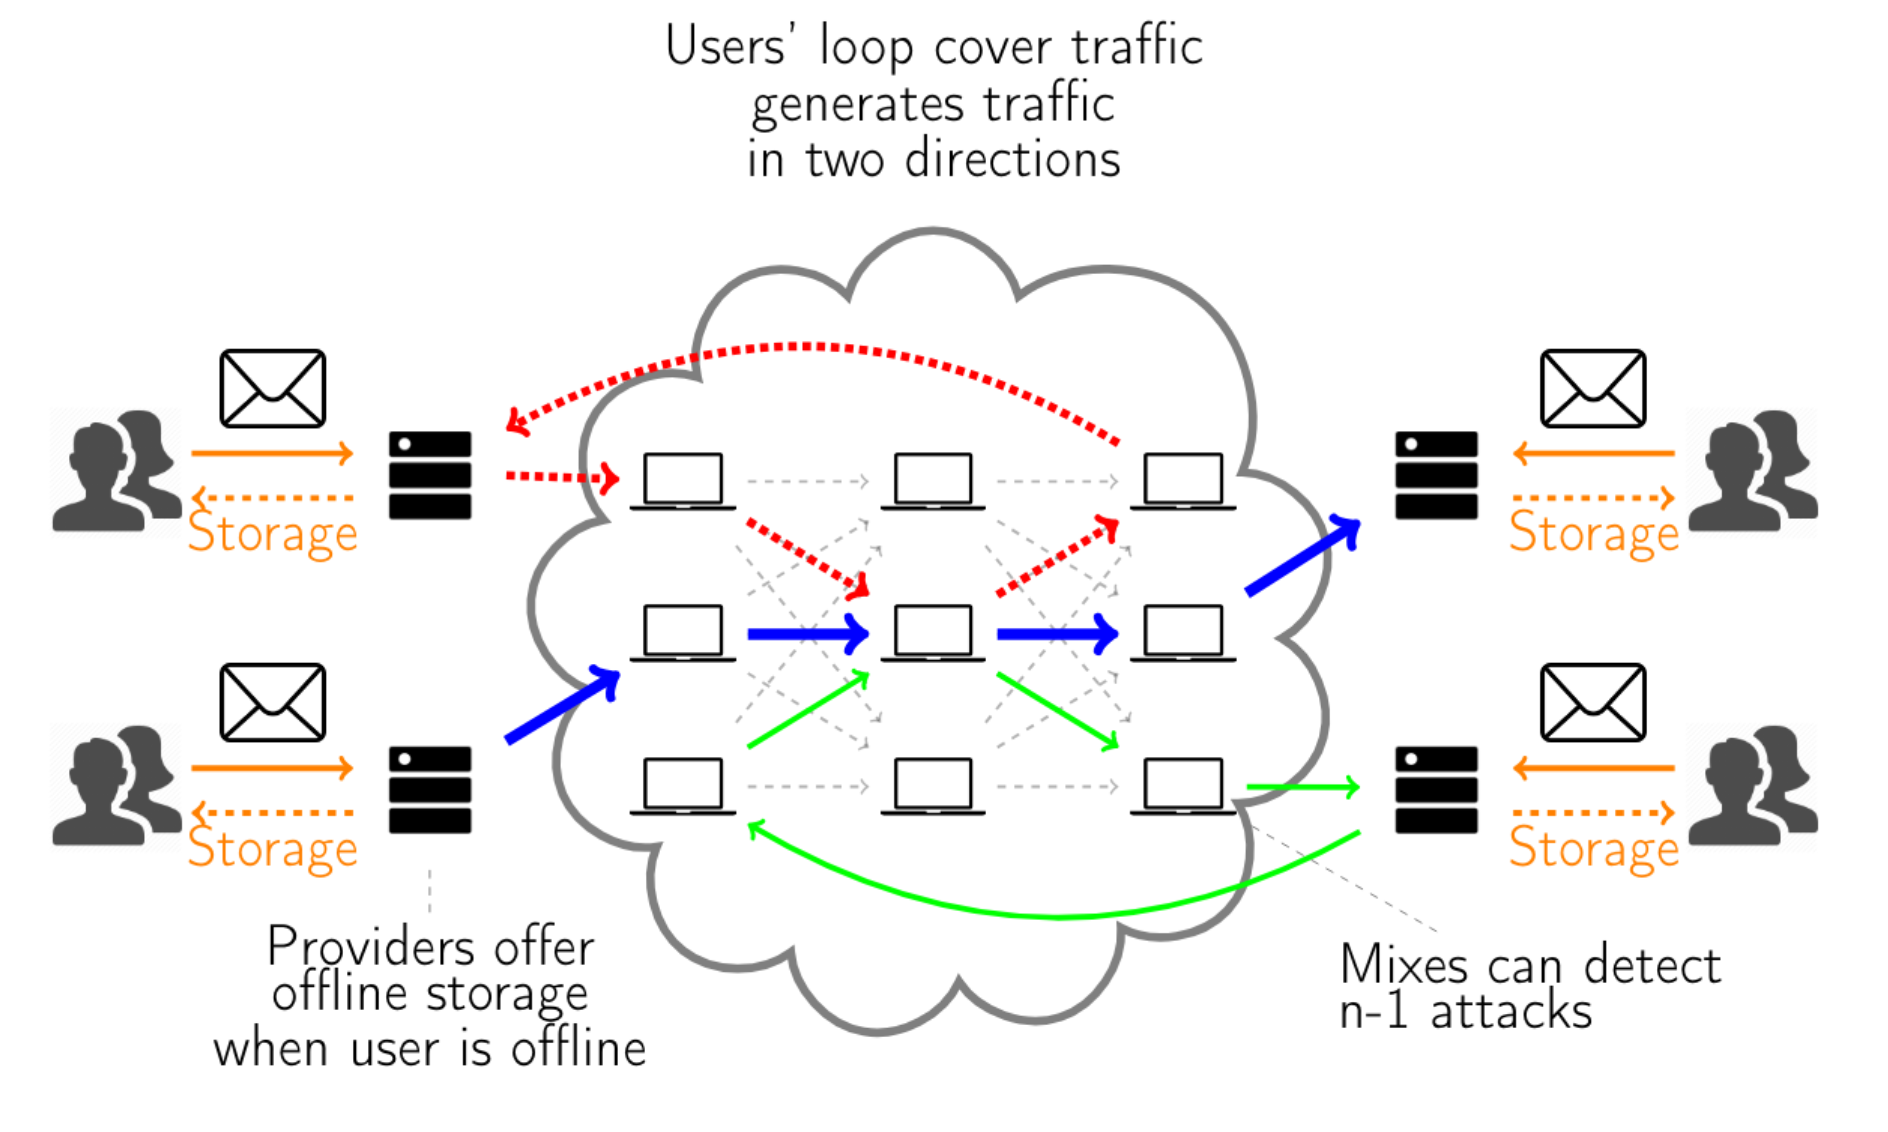
\includegraphics[width=0.8\linewidth]{plots/loopix.png}
    \caption{}
    \label{fig:loopix}
    \small\textit{Figure 1 from The Loopix Anonymity System paper}
\end{figure}

The typical route of a message from the client goes \textbf{provider -> mixnode layer 1 -> mixnode layer 2 to n -> provider of the destination -> destination client}. Of course, this requires the source client to know mixnodes at each layer as well as the destination node and the provider of the destination node.
\textbf{TODO get rid of the text at the top of the figure}

%-------------------
\subsection{Types of Messages}
\begin{itemize}
    \item \textbf{Subscribe Message} \\
    When a client joins the network client sends a subscribe message to a provider of its own choosing. When a provider receives a subscribe message, it simply adds the client to its list of subscribed clients and stores any messages that arrive for this client.
    \item \textbf{Payload Message} \\
    If a client want to send a real message to another client, it creates a payload message. These payload messages are then put into a queue and the client pops messages from this queue at a constant rate.
    \item \textbf{Drop Message} \\
    If the client payload message queue is empty, the client sends a drop message instead. These message are sent to a random random provider and they are dropped at the destination. All nodes, clients, providers, and mix nodes, periodically send drop messages.
    \item \textbf{Loop Message} \\
    Loop messages are the \textbf{namesake of the loopix anonymity system}. They are a part of the cover traffic along with the drop messages. Loop messages are mmessages that a node sends to themselves, routed through a random provider. They mimick getting a reply for a message, and provide important \textbf{security/privacy} properties which will be detailed in the next section.
    \item \textbf{Pull Message} \\
    When a client is online, it periodically asks provider whether the provider is storing any many messages for it. Pull message serves this purpose. When the provider receives a pull message, it will send a predetermined number of messages back to the client. These message messages can be real messages destined to the client, or messages created by the provider to fill up the predetermined number.
    \item \textbf{Dummy Message} \\
    Dummy messages are messages sent to a client by the provider as a response to pull messages, if the provider does not store enough messages. For example, if the provider is storing 3 messages and needs to send 5, it will create 2 dummy messages to \textit{pad} its response.
\end{itemize}

%-------------------
\subsection{Threat Model}
\label{sec:loopix_assumptions}
An adversary can observe all traffic. The mix network prevents sender - receiver linkage. Even with misbehaving providers and all but one mix node misbehaving, loopix provides protections against an adversary observing whether a sender and a receiver are communicating.  \textbf{is this really corrupt provider????}

Particularly at a single mix node, loopix provides strong protection against trickling attacks, where the adversary drops all but one packet and tries to correlate the destination of that packet. Thanks to the presence of drop and loop messages that are sent periodically at each mix node, the adversary cannot know exactly which packet is the one they let into the mix node. \textbf{we will talk about in more detail in the autoref section}. This being said adversary can delay, drop, inject packets into the network with the purpose of learning information about the communications of the honest clients.

\textbf{finish this part}
Message in distinguishability
client-provider unobservability


passive traffic analysis
n01 attack
end to end correlation
sender receiver third party unlinkability: if two parties are commyunicating, GPA (section 4.3), 
sneder online unobservability: adversary doesn't know if A is communicating with B or not, corrupt provider
receiver unobservability: is there communication to B from any sender (4.1.2) honest ptovifrt

\textbf{talk about what is malicioius here}
\begin{itemize}
    \item honest but curious providers
    \item a fractions of mixnodes can be malicous
    \item a fraction of clients can be malicioius
\end{itemize}
%-------------------
\subsection{Parameters}
\begin{itemize}
\item \textbf{Path length} \\
This is the number of hops a packet goes through in the mix node. Although chosen by the clients, the authors of the Loopix paper recommend a path length of 3 or more. Each hop of the packet would be in layer of the mix network topology.
\item \textbf{Mean Delay} \\
This is the average amount of time a packet stops at a mix node. This value is used to draw from the exponential distribution while the a node is creating a packet that will go through the network. For each hop, one value is drawn from this distribution.
\item \textbf{Payload Message Rate (\(\lambda_p\))} \\
The rate at which the clients sends messages from it's "real" message queue. In this project we will use all \(\lambda\) values as \(x\) per second, however \(\lambda\) values can be rates with any time unit.
\item \textbf{Loop Message Rate (\(\lambda_L\))} \\ 
The rate at which each node sends loop messages. Although the Loopix paper distinguishes between the loop message rate of mix nodes (\(\lambda_M\))and clients (\(\lambda_L\)), in this project, for simplicity we will use the same values for both and refer to it as \(\lambda_L\).
\item \textbf{Drop Message Rate  (\(\lambda_D\))} \\
The rate at which all nodes send drop messages. 
\item \textbf{Time-to-Pull} (\(t_{pull}\))\\
This is the amount of time that a client waits between each pull message to its provider. Although not explicitly defined in the loopix paper, it can be found in the reference implementation \textbf{cite} by the authors. In this project we will use seconds to define this value.
\item \textbf{Number of messages retrieved (\(N_R\))} \\
The number of messages the provider sends each time it receives a pull request. It always sends this number of messages to ensure that an adversary cannot tell whether a client is receiving messages or not. If there aren't enough messages for the client, it will also send dummy messages to make sure exactly \(N_R\) messages are in its response. Again this parameter is not explicitly defined in the Loopix paper, but can be found in the reference implementation.
\end{itemize}

\subsubsection{Mean number of messages in a mix node}
\label{sec:lambda_over_mu}
An important security parameter is the mean number of messages in a mix node at a given time. This is essentially number of messages that are being "mixed" at the mix node at a time. An adversary can observe some messages coming into the mix node, it waits a certain amount of time and observes some messages leaving the mix node. It is  \textbf{TODO complete this}
It is an estimate where lambda is the number of incoming messages every second. And mu is the inverse of the mean delay. One can thing of it as the number of messages that are "leaving" the mixnode on average per second. It is important to note that this estimate assumes that there are no loop messages \textbf{and drop?} being send by the mixnode. The Loopix paper recommends lambda/mu of 2. 

%%%%%%%%%%%%%%%%
\chapter{Design}
%%%%%%%%%%%%%%%%

% Introduce and discuss the design decisions that you made during this project.
% Highlight why individual decisions are important and/or necessary. Discuss
% how the design fits together.

% This section is usually 5-10 pages.
%-------------------
\section{Choosing an Anonymous Communication System}
\label{sec:mixers}
%-------------------
Having identified our initial goal, namely making Fledger web proxy more privacy preserving, the first step was to find a suitable mix network or more broadly an anonymous communication system that can be used in the context of browsing the web through a web proxy. For this purpose, we identified potential anonymous communication systems to look into. This section will detail the process of choosing Loopix to integrate into Fledger, and the reasoning behind this choice.

\subsection{Atom}
Development of a scalable anonymous messaging system that defends against traffic analysis attacks. The system is very scalable and techinically over a million users are supports with \textbf{talk about privacy qurantees}, they only achieve 28 minute latency. THis latency might be acceptable for an aync messaging application however, for accessing web pages, this is not usable.

\subsection{Riffle}
Development a bandwidth- and computation-efficient anonymous communication system resistant to traffic analysis. \textbf{talk a bit more about the papers here?} Less than 10 second latency with 100000 users with 100KB/s per user in file sharing applications.  Although 10 seconds is much better than 28 minutes, we are still looking for something that can be more usable for a web proxy. And for the future file sharing applications of fledger 10KB per second would not be enough for a real system.
\subsection{Vuvuzela}
Develop a scalable and flexible metadata-private messaging system that allows asynchronous communication across multiple devices. 37 second latency still not what we are looking for. 
\subsection{Grove}
latency of 32-80 seconds , not enough. Also the focus of the paper was having a an async communicatoin across multiple devices not really latency
\subsection{Prifi}
Low latency DC net with 100ms latency, but only supports up to 100 clients. 

\subsection{Loopix}
As we have talked about Loopix we will not go into further detail here. We chose loopix for it's low latency, scalability, availablility of reference implementations and the tunability of the system. There are also many works that have built on top of loopix which attests to it's extensibility, such as larmix which uses latency aware routing to reduce the network latency between nodes. \textbf{make this a better paraphraph}.

%-------------------
\section{Loopix Integration into Fledger}
%-------------------
\subsection{Loopix as a fledger module}
\autoref{sec:fledger_modules} goes into detail how Fledger contains many modules and is very extensible. Keeping this in mind, we set out to create a Loopix module that can fit between any Fledger module and the network. Although primary focus of this project has been, using the Loopix module as an intermediary between the web proxy module and the network, Fledger Looopix module described in this section has been designed to work with other modules.

Here is how it works. When a node wants to use web proxy through loopix module, it will create the web proxy module with loopix overlay. Loopix overlay translate the message into a a format that loopix module can understand, note that it could be any fledger module that can send a message to loopix overlay to be translated. Note that only Loopix Clients can send web proxy requests. When loopix module receives a message from overlay it will create a route that goes through its own provider, the mixnetwork, the destion clients provider and finally the client that will be the web proxy. Once the route is created it will create delays for each mixnode. And then encrypt using the public keys of each node. Kind of like onion routing.

Loopix module will then send the encrypted message to network module with the destination as the next node in the route, network module will send it to the destination.

The next node receives the node message in the network module, network module sends the message to loopix module and the loopix module will unwrap one layer from the encryption (provided that it is indeed the correct node that receives the message). This next layer of information contains routing information (only to the next node) as well the specific delay to wait. After waiting the delay, this node sends the message to the network module and so on, until the message eventually reaches the provider of the final destination.

When the provider unpacts the message, it check if the next hop is one of its clients. If so, instead of sending this message directly it stores the message in its own storage until the client asks for messages. When the provider receives a pull request it will send the message along with all the messages in it's storage (it does keep track of the messages it has sent), and if there isn't max retrieve messages to send it will send dummy messages.

Finally the client receives the web proxy request. Through the network module, the network module will peel the final layer of encryption and recover the plaintext, which is a message from the overlay, it will be sent to overlay module, which will in turn translate it into a web proxy message.
\textbf{THE ORIGIN ID IS THERE SO THE PROXY KNOWS WHOS ACCESSING WHICH MESSAGE AGAIN!!!!!!!!!!}
\textbf{BUT this can easily be remedied with the single use reply blocks}

The web proxy module receives the request, gets the url requested and sends all the messages back towards the originator of the request through the network module. And then we go through all the hops again until the provider of the originator etc.

\begin{figure}[H]
    \centering
    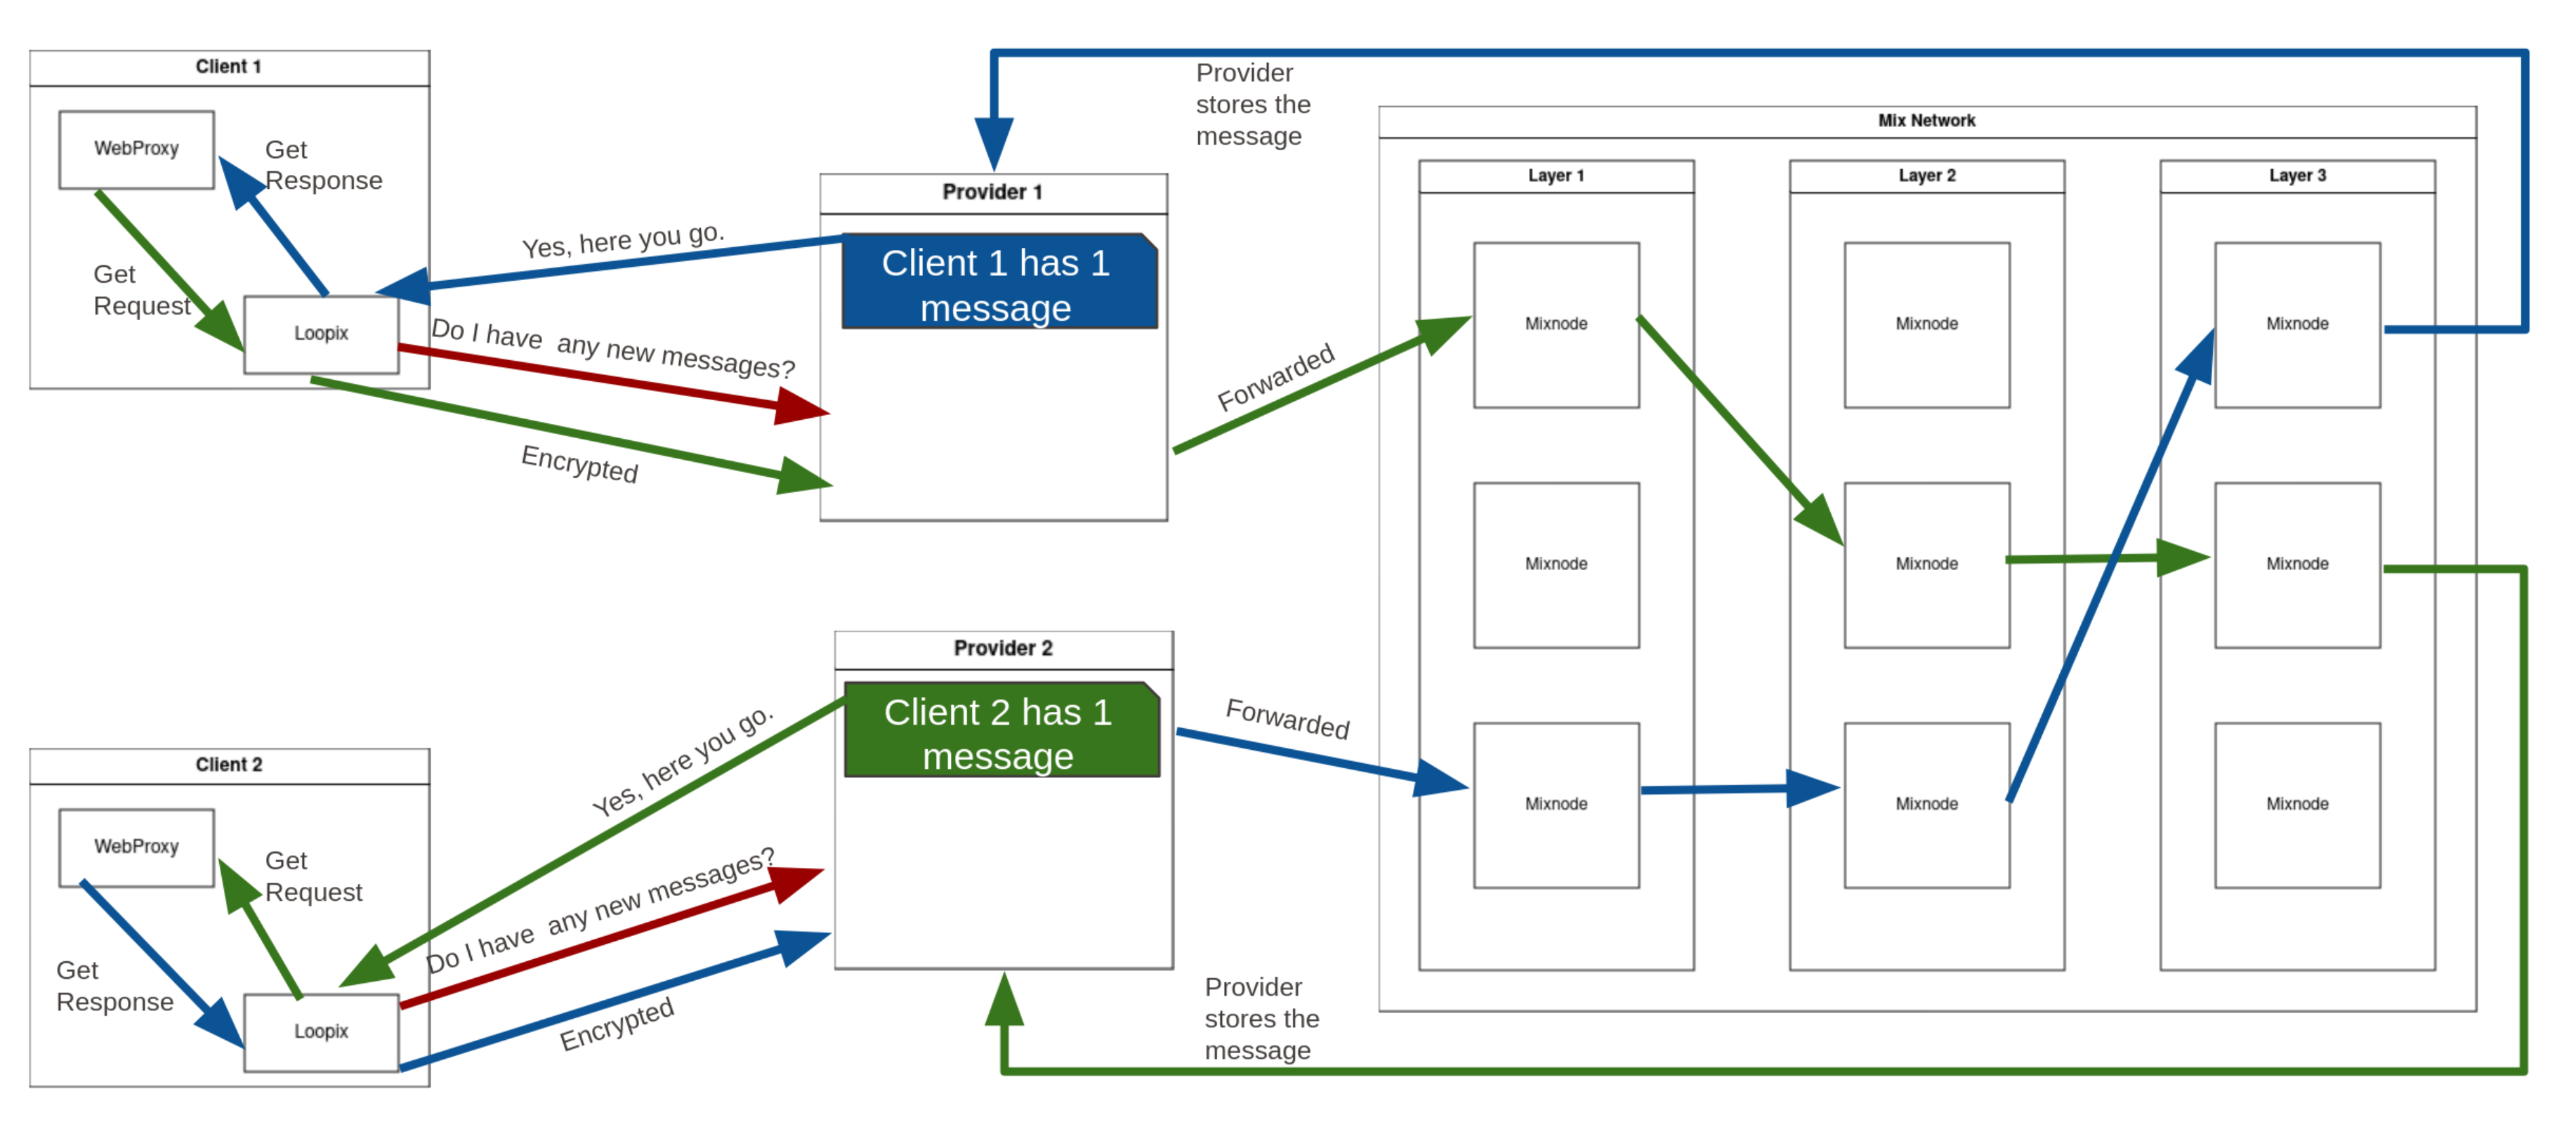
\includegraphics[width=1\linewidth]{plots/implementation.png}
    \caption{}
    \label{fig:implementation}
\end{figure}

%-------------------
\subsection{Assumptions}

For the most part
Web proxy => web page access patterns
Every time a node goes online, a specific website is accessed
Enough users to provide an anonymity set
Providers know usage patterns
They are “trusted”

%-------------------
\subsection{Bootstrapping}
- signalling server
- nodeID in message
- even unique message ID
Fledger Signaling Server (WebRTC)
Tells nodes which other nodes are online (!)
\textbf{talk about how we can get rid of providers}


\section{Potential Approaches to More Reliable Message Delivery}
\label{sec:reliable_message_delivery}
\textbf{Talk about the simple approach, retrying and duplicate messages}
\textbf{Talk about }

\section{Further Adaptation to Fledger}

\section{Future Work}

%%%%%%%%%%%%%%%%%%%%%%%%
\chapter{Implementation}
%%%%%%%%%%%%%%%%%%%%%%%%

% The implementation covers some of the implementation details of your project.
% This is not intended to be a low level description of every line of code that
% you wrote but covers the implementation aspects of the projects.l

% This section is usually 3-5 pages.
\section{Communication between Modules}
\textbf{Talk about messages and how they wrapped between modules}

\section{Performance Improvements}
\textbf{Two big performance improvements: parallel message processing, stop adding each message to storage :)}

\section{Miscellaneous}
\textbf{Talk using rust sphinx for messages and the one line adaptation needed (maybe I need to talk about it in the background)}

\textbf{Talk about one caveat with duplicate messages: web proxy cannot avoid reprocessing (duplicate) responses, it doesn't know how many packets it will receive}

%%%%%%%%%%%%%%%%%%%%
\chapter{Evaluation}
%%%%%%%%%%%%%%%%%%%%

% In the evaluation you convince the reader that your design works as intended.
% Describe the evaluation setup, the designed experiments, and how the
% experiments showcase the individual points you want to prove.

% This section is usually 5-10 pages.

\textbf{I will rerun some weird points}
%-------------------
\section{Experiental Setup}
%-------------------
Talk about setup etc and how I wasn't able to setup a massive experiment

number of nodes,
nnetwork latency bandwidth links
nodes operating system cores ram

Experiments where run with 3 clients 6 mix nodes with path length of 3 (2 mixnodes per layer), and 3 providers. With a 50 mbps link between each node with 15ms latency (fully connected). Although in an ideal scenario, this experiment would run with many more nodes with one link connecting to a router node, due to connectivity issues between nodes on the network level as well as lack of documentation in sphere testbed, this has not been possible. However, we still hope to convince the reader of the scalability of the system by the end of this section. 

\textbf{add figure here}

Each node runs Ubuntu 20.04 LTS with 4 GB RAM and 4 cores on Sphere Testbed \textbf{cite?}. The signal node is running 32 RAM and 32 cores to make sure that it is indeed not a bottleneck.


\textbf{Talk aboout the setup and what the nodes are doing during the experiment for how long, how many proxy requests over the 5 mins.}
\begin{figure}[H]
    \centering
    \includegraphics[width=\textwidth]{plots/experimental_setup.png}
    \caption{}
    \label{fig:setup}
\end{figure}

%-------------------
\section{Fine tuning Loopix Parameters for Web Proxy}
\label{sec:finetune}
%-------------------
In section this section, each measurement is taken within a simulation of 5 minutes. The nodes are allowed get started for 15 seconds, after which Fledger Loopix module is started. Here the web proxy timeout mentioned in \textbf{autoref} is set to 20 seconds. This ensures that each request takes as long as it needs, and any proxy request that is not successful means dropped packets or \textbf{something along those lines.}
%-------------------
\subsection{Mean number of messages in the mix}
As mentioned in \autoref{sec:lambda_over_mu}, one important security parameters for loopix system is the mean number of message in the mix. One issue with the Loopix paper is that in their experiments, they used providers and mixnodes with essentially unlimited resources. \textbf{Quote from the paper here}. Which makes it easy to reach their recommendation of lambda over mu.

However, Fledger is designed as a lightweight program, user that want to participate in as mixnode should not need to have \textbf{X amount of RAM and Y cores}. And so keeping in mind that the lambda over mu estimate does not take into account loop messages and the fact that using loopix as already gives up some privacy properties of the original system, we first look into choosing a suitable value for the incoming that a \textbf{low specced machine} can handle.

In this section we keep all parameters of the loopix system stable expect the \textbf{lambda loop drop} etc. This is used to adjust the incoming messages per second while keeping the latency the same, which in turn changes the value of the mean number of message in the mix the mix.

The mean delay is set to 100ms which correcsonds to a 1/mu of 1/10, so according to the loopix paper, the target value incoming messages per second is 20. lambda/mu = 2. \textbf{with payload =6?}

\begin{figure}[htbp]
    \centering
    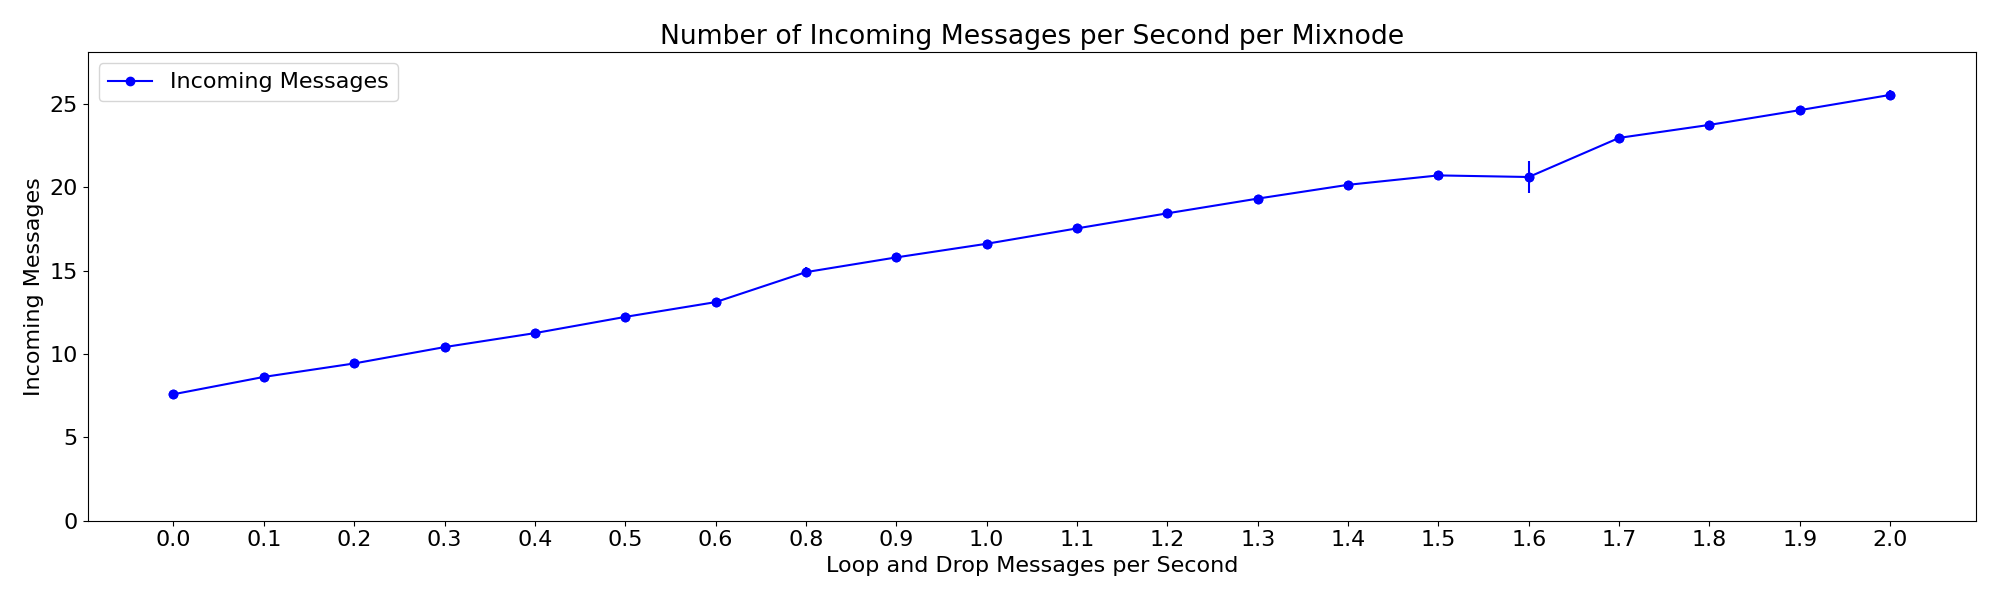
\includegraphics[width=\textwidth]{plots/mu_incoming_messages.png}
    \caption{}
    \label{fig:mu_incoming}
\end{figure}

\begin{figure}[htbp]
    \centering
    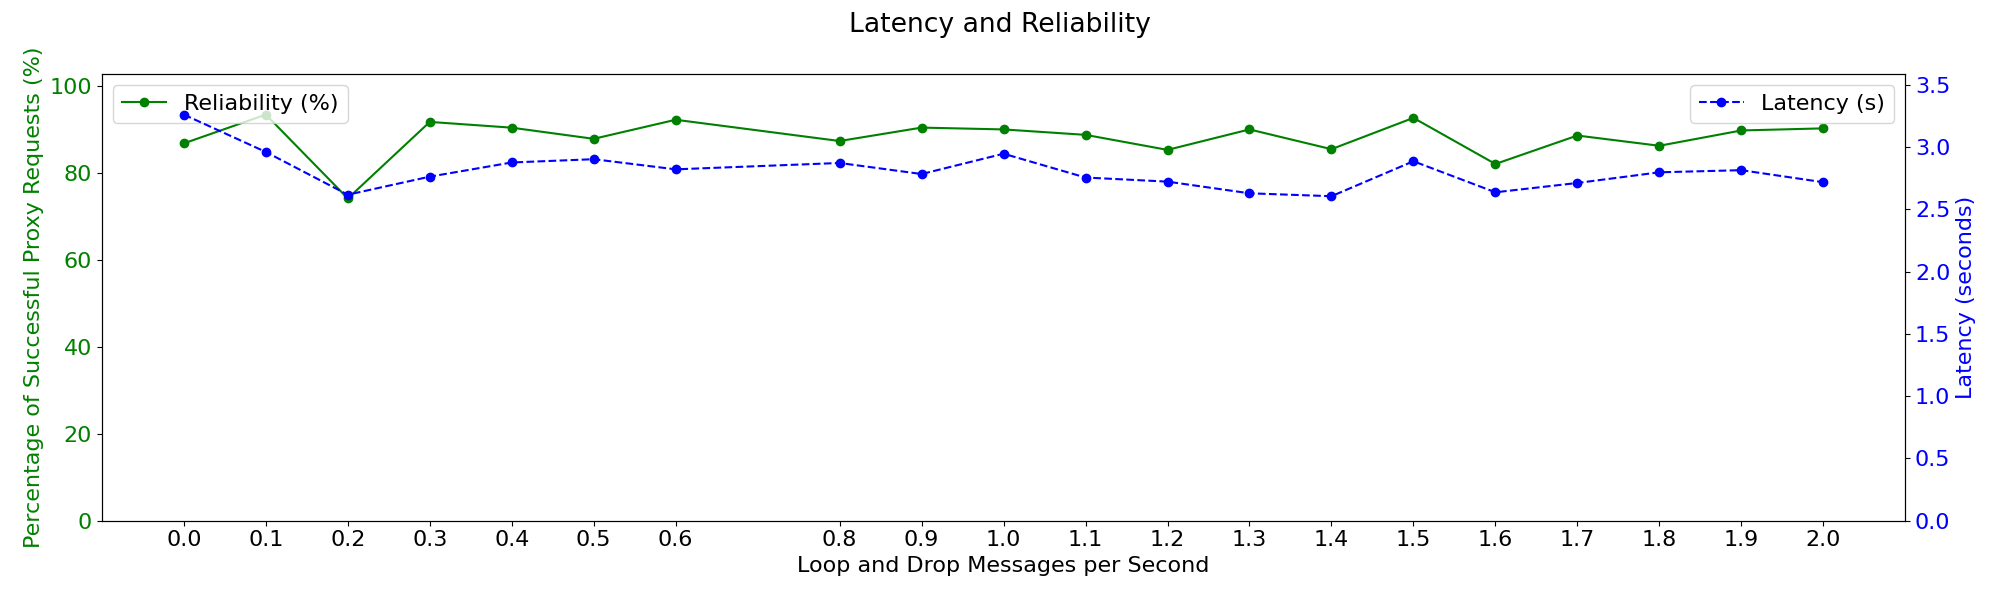
\includegraphics[width=\textwidth]{plots/mu_reliability_latency.png}
    \caption{}
    \label{fig:mu_reliability_latency}
\end{figure}

In \autoref{fig:mu_incoming}, we see that we can adjust the value of the the incoming messages by only adjusting the the cover traffic rates, and in \autoref{fig:mu_reliability_latency}, we see that adjusting the incoming message rate does not affect the reliability the end to end latency of the system.

\textbf{say something about randomness and the measurement is approximate}
This let's us use the recommended lambda/mu value of 2.

%-------------------
\subsection{Latency Components}
It is important to talk about what contributes to the end to end latency of a proxy request. We will show these components through a control run, where all configuration parameters are the same and the simulation is run 12 times for 5 minutes. While showing that given a certain configuration, the system latencies are quite stable, it is important to note that there is a variation of 200-400ms between the averages of run. 

\textbf{talk about the different components that contribute to the end to end latency}

\begin{figure}[htbp]
    \centering
    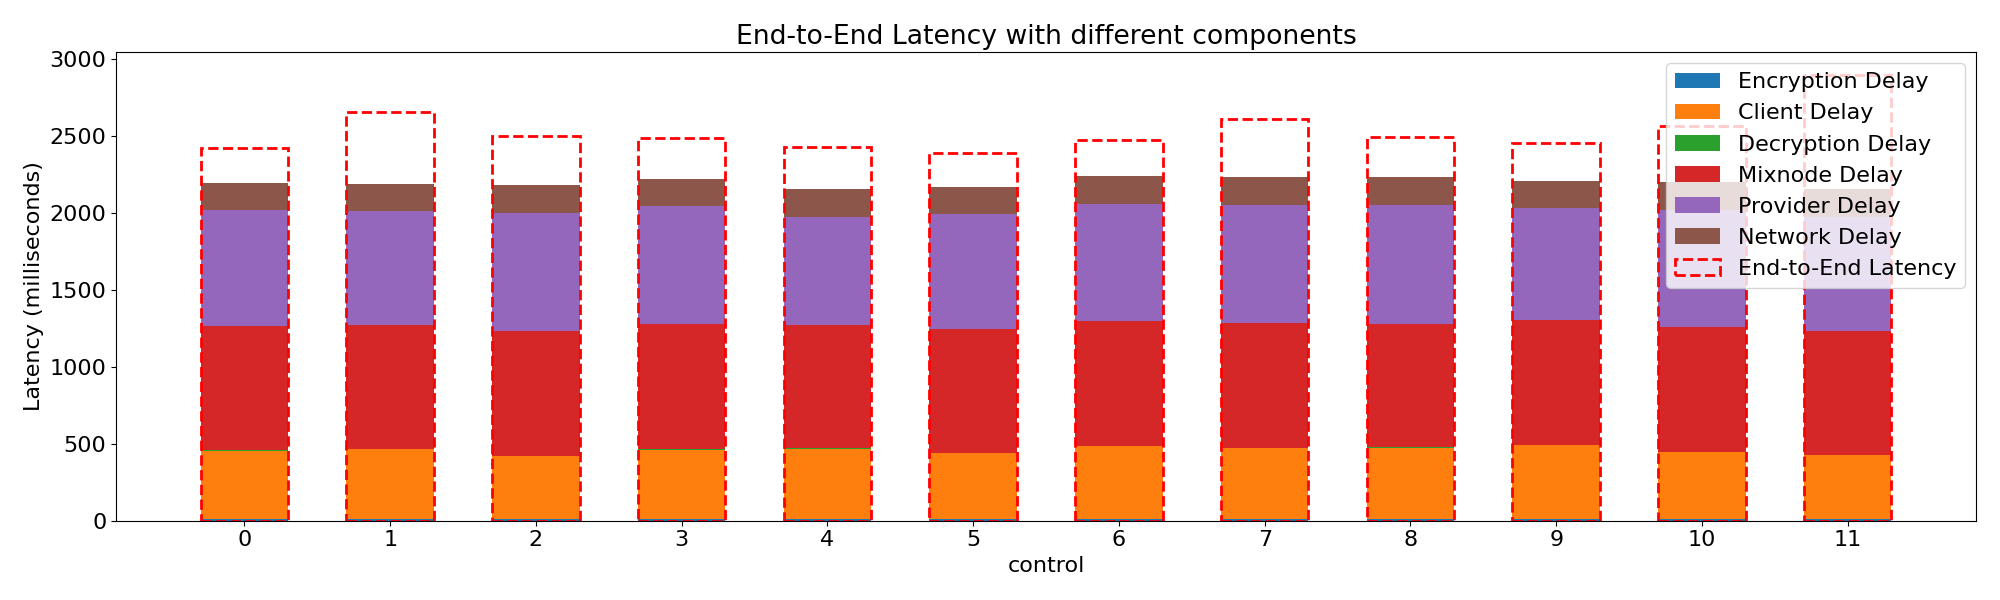
\includegraphics[width=\textwidth]{plots/control_latency_components.png}
    \caption{}
    \label{fig:control_lambdas}
\end{figure}

In \autoref{fig:control_lambdas} each stacked bar represents the average end to end latency in each simulation of 5 minutes. The dotted red line being the actual end-to-end latency, it is slightly higher than the combination of all the listed components, these components are are parts of the loopix configuration (plus network delay) and everything between the dotted red line and the bars are things like the time for a proxy node to get a website, for the nodes to prepare and send web rtc messages between each other etc. Looking at the figure, one can see 4 big components that contribute to the end-to-end latency.

\begin{itemize}
    \item \textbf{Client Delay} \\
    This is the time that a message waits in the client queue after being created. The system parameter that it corresponds  to lambda paylaod \textbf{autoref{}}. 
    \item \textbf{Mixnode Delay} \\
    This is how long the message spends time being "mixed", namely the total amount of time it is delayed at each layer of the mix network. It more or less corresponds to number of layers in the mix network + 1 (provider of the initiating client) * mean delay \textbf{autoref}
    \item \textbf{Provider Delay} \\
    This is the amount of time the message spends time at the storage of the (end provider) before being sent to the client with a pull requeset reply. It is affected mostly by time pull \textbf{autoref} and a bit by maxretreive parameters.
    \item \textbf{Network Delay} \\
    The amount of time a packet spends traveling between nodes. In our emulated network, the network delay is set to 15ms, which corresponds to 15 ms per hop, which is path length + 4. 
\end{itemize}

\autoref{fig:control_lambdas} shows the averages of these values over the course of the simulation for both ways. It is also posisble to see decryption delay and encryption delay in the \textbf{legend} of the graph, which are total amount of time decrypting the sphinx packets and total amount of tiem to encrypt the payload messages respectively, however as they contribute to a very small amount of the end-to-end latency, they are not very visible on the stacked bars. 
It is also important to note one caviat with these measurements. For mixnode and decrytion delays, the values are average time for all (including cover traffic) as it is not possible for a mixnode to tell the difference between a payload or a cover message.

%-------------------
\subsection{Lambda Payload and Mean Delay}
As the most binding limitation in our setup is the end to end latency (a user should be able to surf the internet without waiting too long). In this we section try to find mean delay and lambda payload values that reduces the end to end latency without comprimising too much bandwidth\textbf{(!}.

\textbf{Talk about how incoming messages per second is calculated}

\textbf{Talk about the timeout!}

\subsubsection{Lambda payload}

First we adjust the payload value, this warrants a change in the cover traffic rate to keep the mean number of messages one mixnode stable. \textbf{Here we use these values: }

In \autoref{fig:lambdas_latency} one can see that as payload rate increase the client delay, so the latency decrease, however after a payload rate of 6 messages per second the returns are diminishing. We believe this stems from the fact that creation of these packets puts a a load on the client and the provider. This is supported by \autoref{fig:lambdas_realibility} where as the payload increases the success rate of a web proxy request decreases possibly due to dropped packets.

In \autoref{fig:lambdas_bandwidth}, we see that increasing the payload rate increases the bandwidth marginally. And \autoref{fig:lambdas_messages} shows that increasing the payload rate while adjusting the cover traffic does lead to a stable number of incoming messages per mixnode.

\textbf{TODO: I NEED TO RERUN SOME OF THESE}

\begin{figure}[htbp]
    \centering
    \begin{subfigure}{\textwidth}
        \centering
        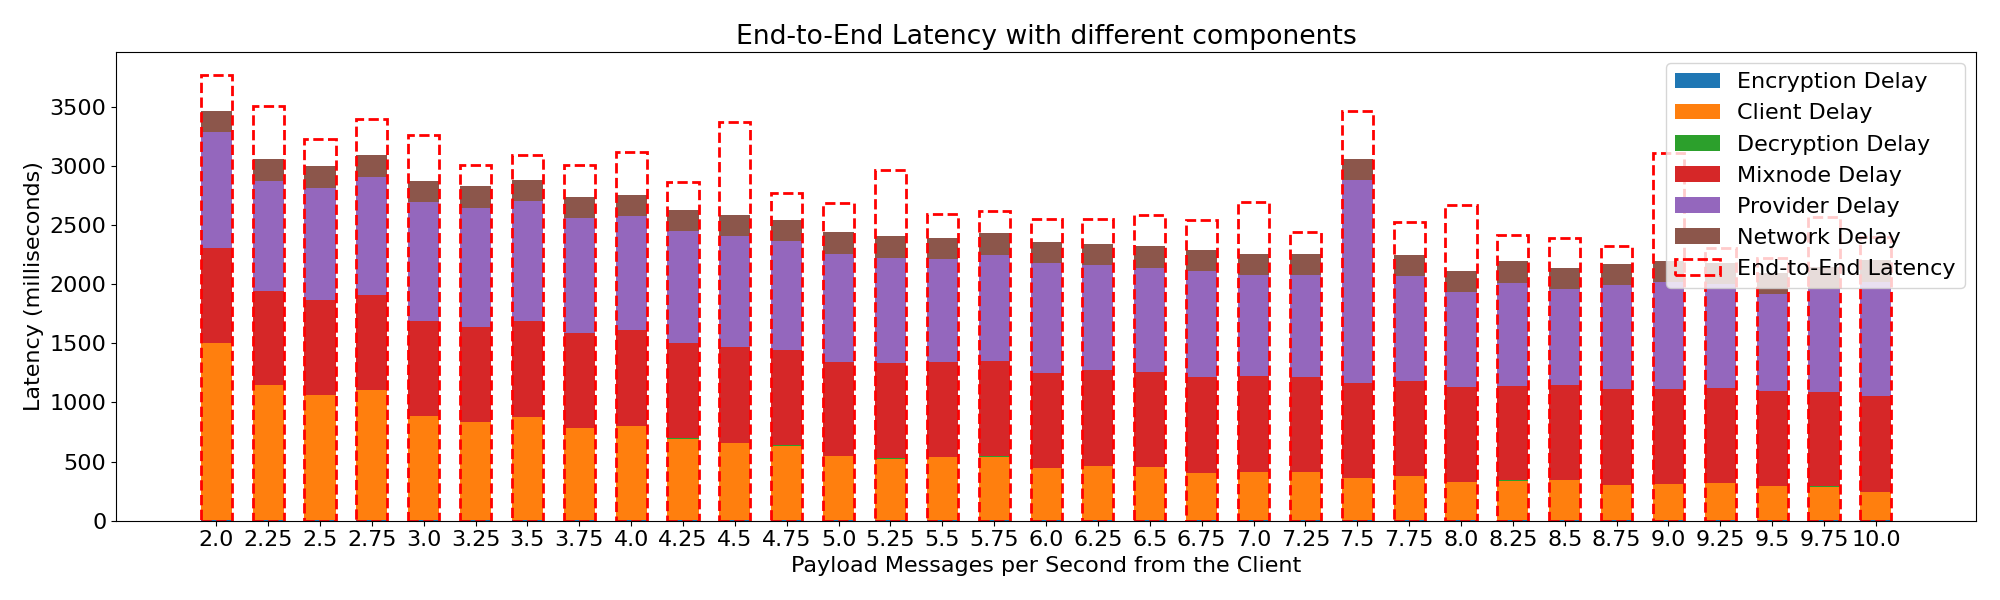
\includegraphics[width=\textwidth]{plots/lambdas_latency_components.png}
        \caption{}
        \label{fig:lambdas_latency}
    \end{subfigure}
    \hfill
    \centering
    \begin{subfigure}{\textwidth}
        \centering
        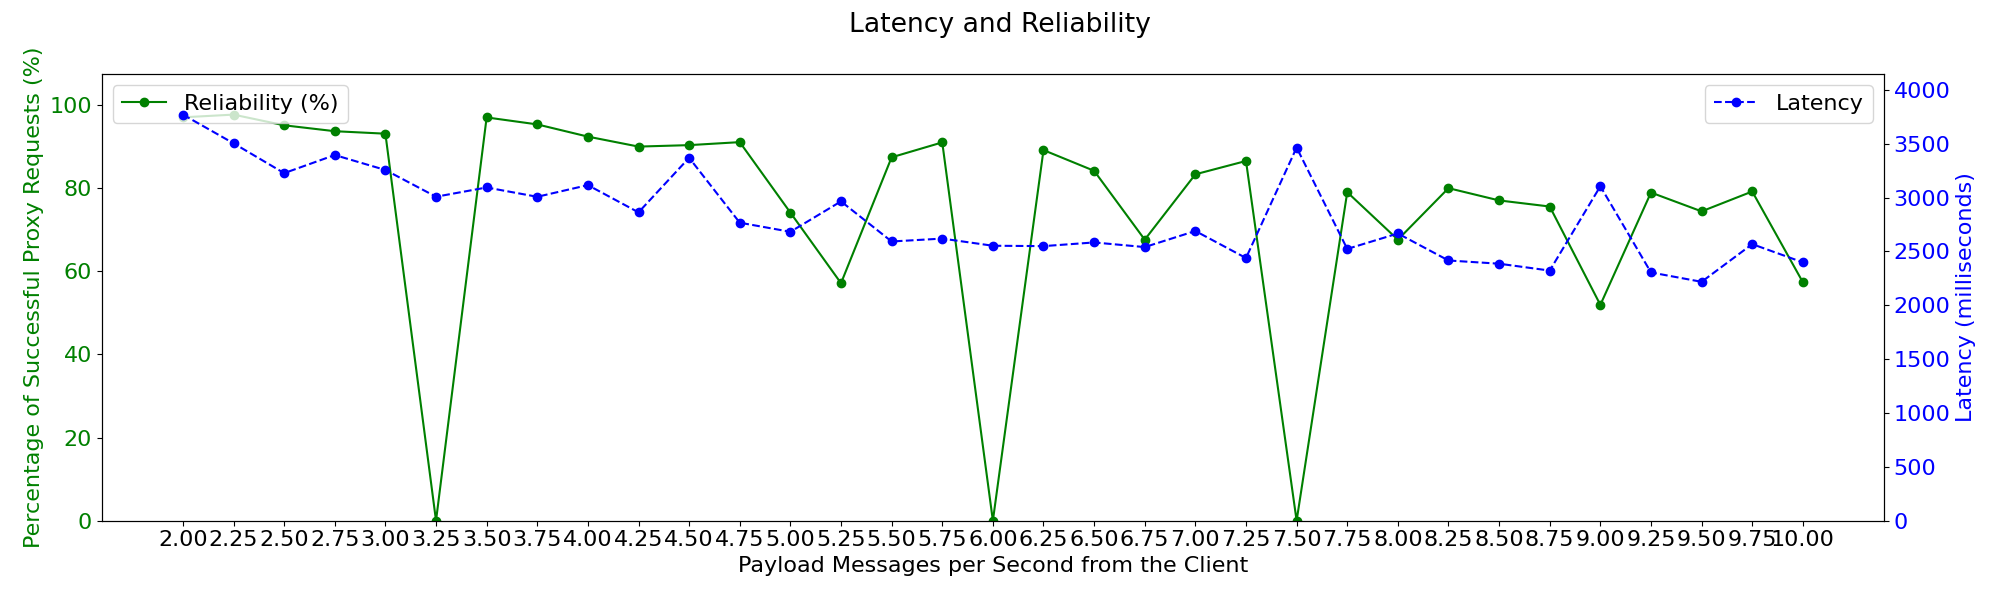
\includegraphics[width=\textwidth]{plots/lambdas_reliability_latency.png}
        \caption{}
        \label{fig:lambdas_realibility}
    \end{subfigure}
    \hfill
    \begin{subfigure}{\textwidth}
        \centering
        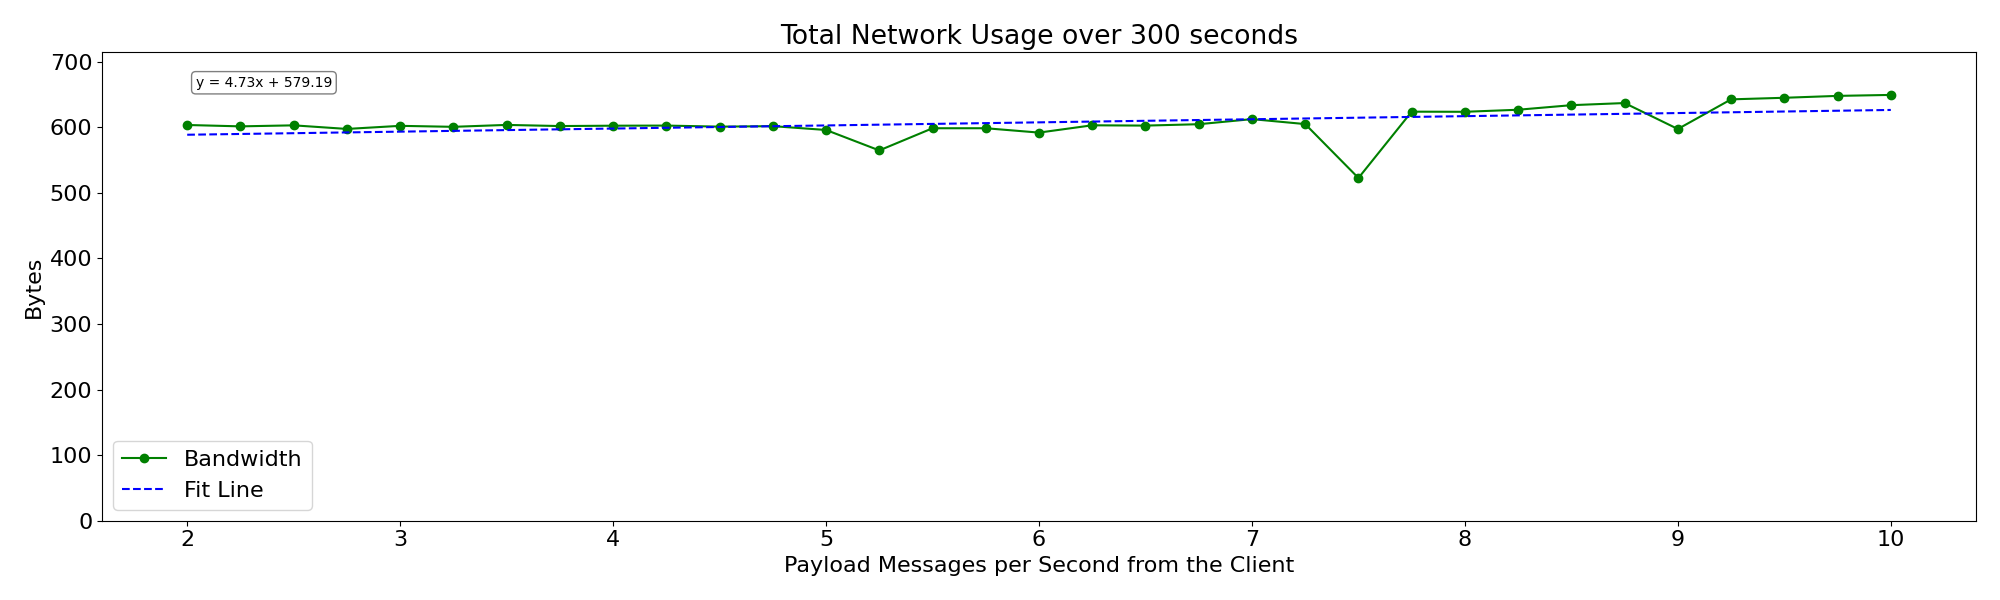
\includegraphics[width=\textwidth]{plots/lambdas_bandwidth.png}
        \caption{}
        \label{fig:lambdas_bandwidth}
    \end{subfigure}
    \hfill
    \begin{subfigure}{\textwidth}
        \centering
        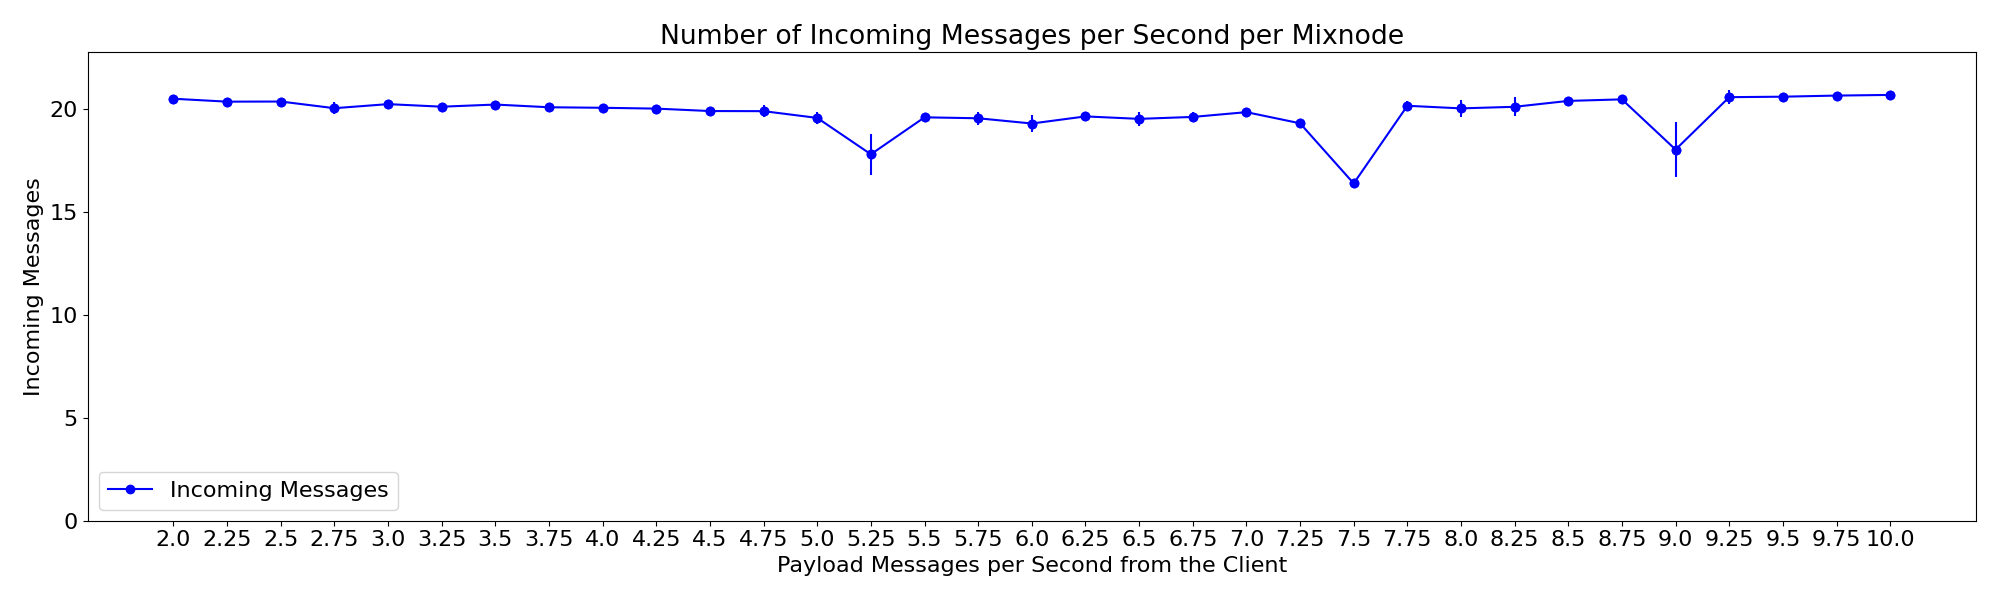
\includegraphics[width=\textwidth]{plots/lambdas_incoming_messages.png}
        \caption{}
        \label{fig:lambdas_messages}
    \end{subfigure}
    \caption{Data Visualization for different payload rates}
\end{figure}


\subsubsection{Mean Delay}
Next we change mean delay values to see how they change the latency bandwidth etc. Unlike, increasing the payload rate, decreasing the mean delay surprisingly increases reliability. We believe this is due to the worker pool mentioned in \textbf{autoref}, for each forwarded packet a thread is spawned, and this thread is part of the worker pool, therefore less time for the delay means less time for the worker to be released.

\begin{figure}[htbp]
    \centering
    \begin{subfigure}{\textwidth}
        \centering
        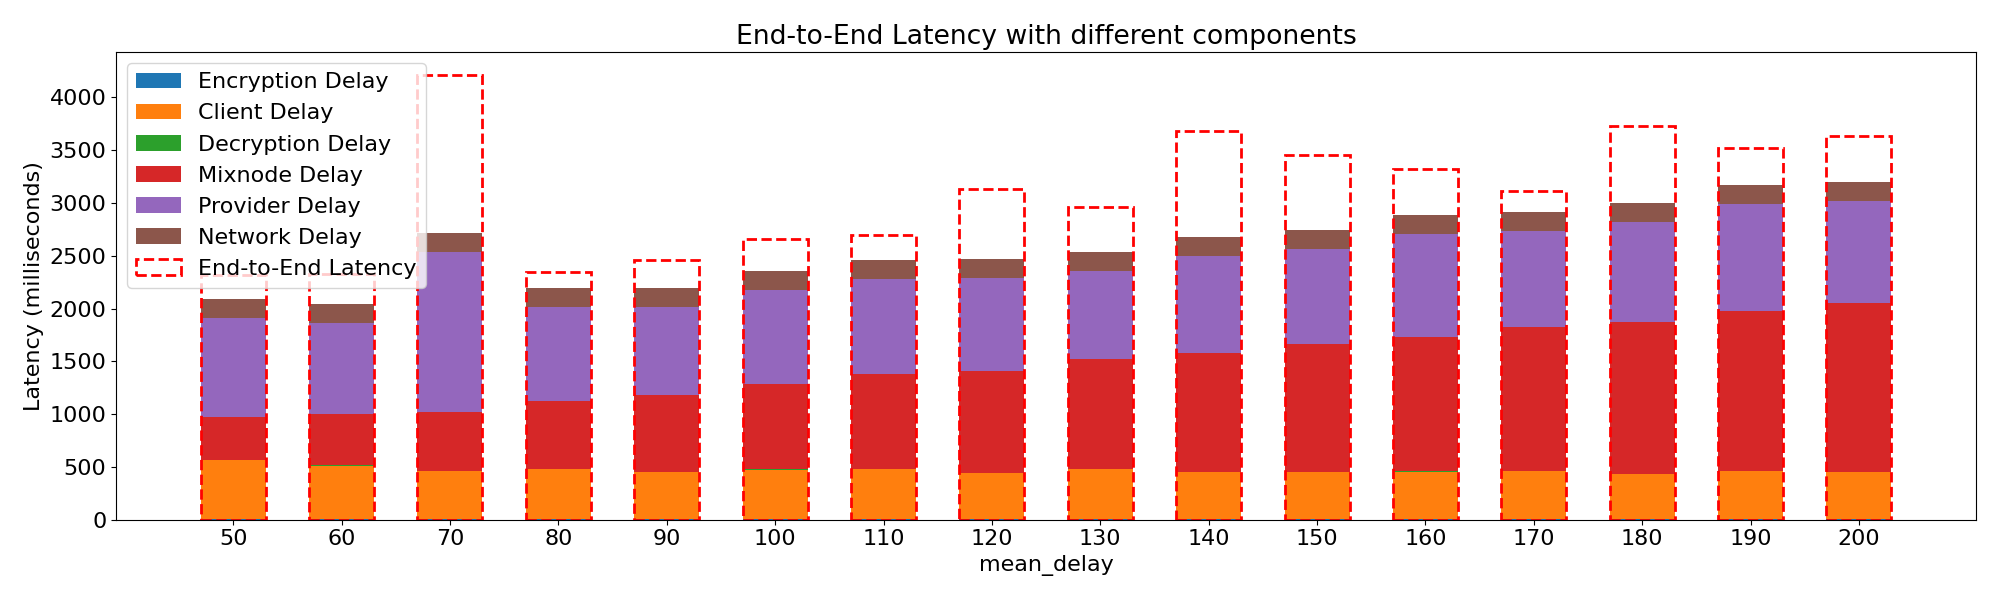
\includegraphics[width=\textwidth]{plots/delays_latency_components.png}
        \caption{}
        \label{fig:lambdas_latency}
    \end{subfigure}
    \hfill
    \centering
    \begin{subfigure}{\textwidth}
        \centering
        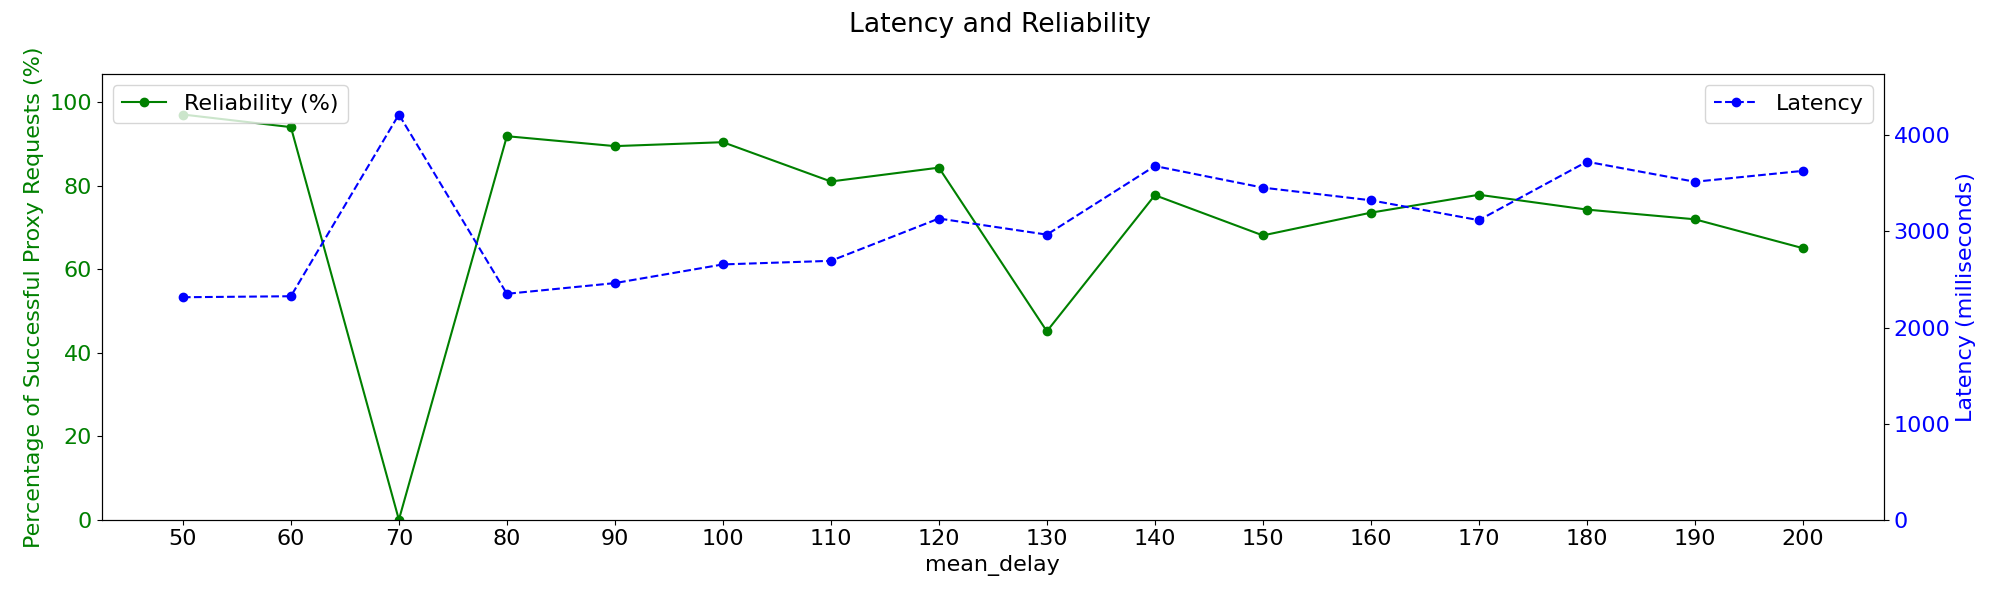
\includegraphics[width=\textwidth]{plots/delays_reliability_latency.png}
        \caption{}
        \label{fig:lambdas_realibility}
    \end{subfigure}
    \hfill
    \begin{subfigure}{\textwidth}
        \centering
        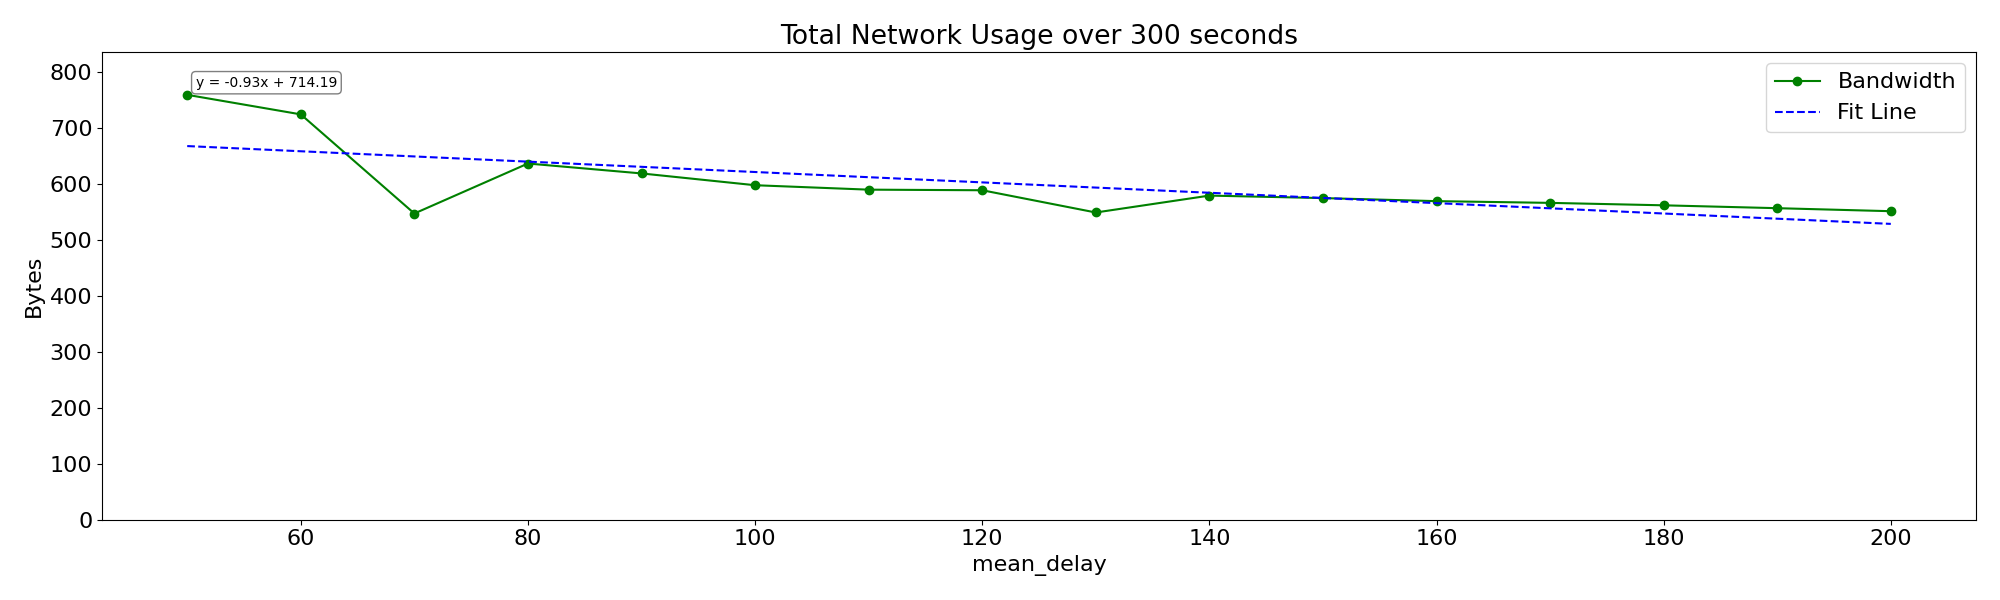
\includegraphics[width=\textwidth]{plots/delays_bandwidth.png}
        \caption{}
        \label{fig:lambdas_bandwidth}
    \end{subfigure}
    \hfill
    \begin{subfigure}{\textwidth}
        \centering
        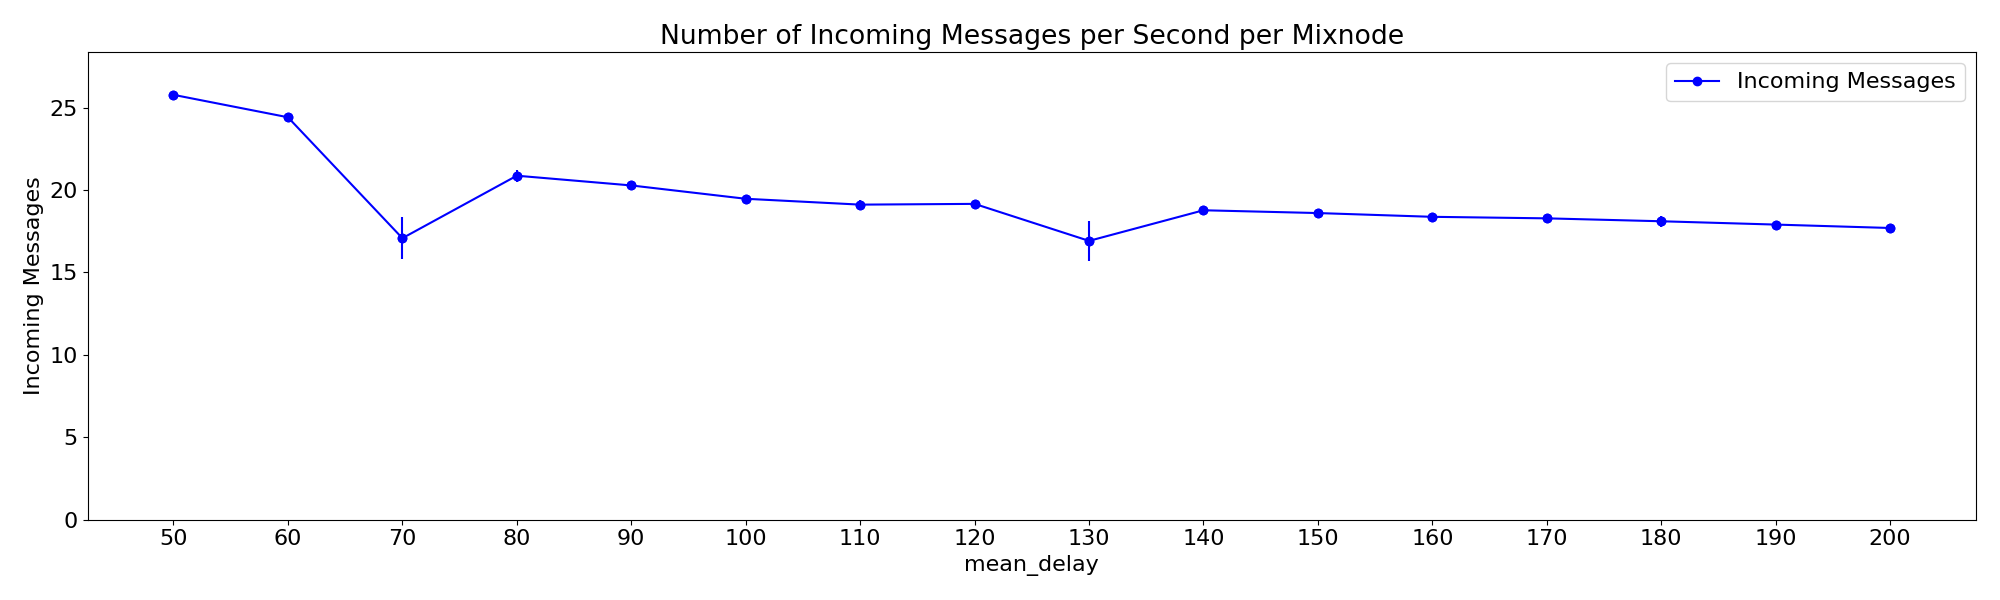
\includegraphics[width=\textwidth]{plots/delays_incoming_messages.png}
        \caption{}
        \label{fig:lambdas_messages}
    \end{subfigure}
    \caption{Data Visualization for different mean delays}
\end{figure}

Since latency decreases and reliability increases, and bandwidth is not affected \textbf{technically shouldn't affected anyway, but I need to rerun a few with less chaff traffic}, we choose 60 as the mean delay going forward. \textbf{link to figures}

%-------------------
\subsection{Choosing Max Retrieve and Time pull}

The final big component that contributes to end-to-end latency is provider delay. As mentioned in \textbf{autoref}, this delay is relatex two max retreive and time pull. This section shows the results of a grid search to find a good compromise betwen latency and bandwidth.

In figure \textbf{autoref} there are two heatmaps, one that shows how max retreive and time pull affects total bandwidth and one that shows how these two variables effects end to end latency.
\begin{figure}[htbp]
    \centering
    \begin{subfigure}{\textwidth}
        \centering
        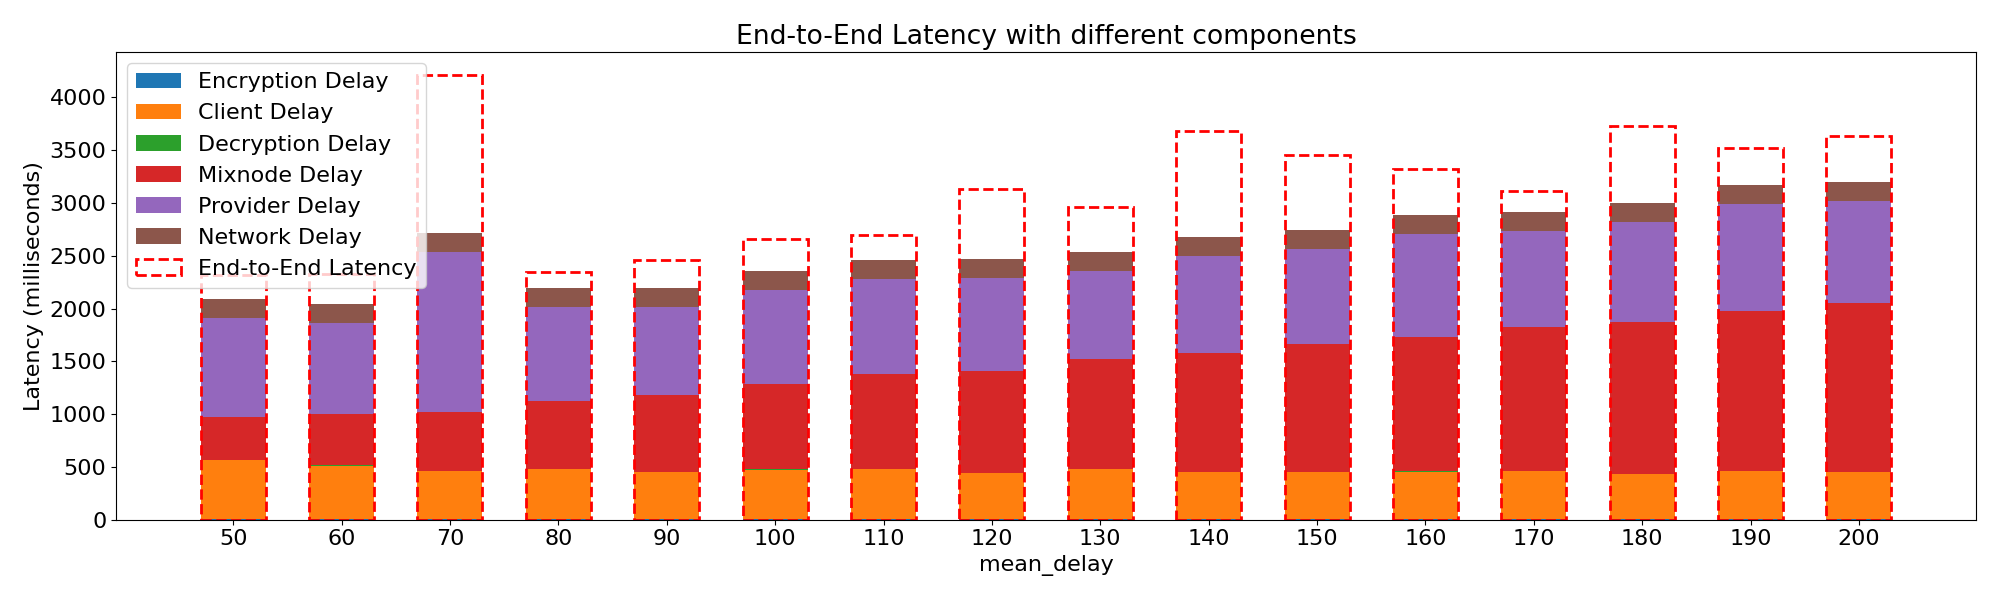
\includegraphics[width=\textwidth]{plots/delays_latency_components.png}
        \caption{}
        \label{fig:lambdas_latency}
    \end{subfigure}
    \hfill
    \centering
    \begin{subfigure}{\textwidth}
        \centering
        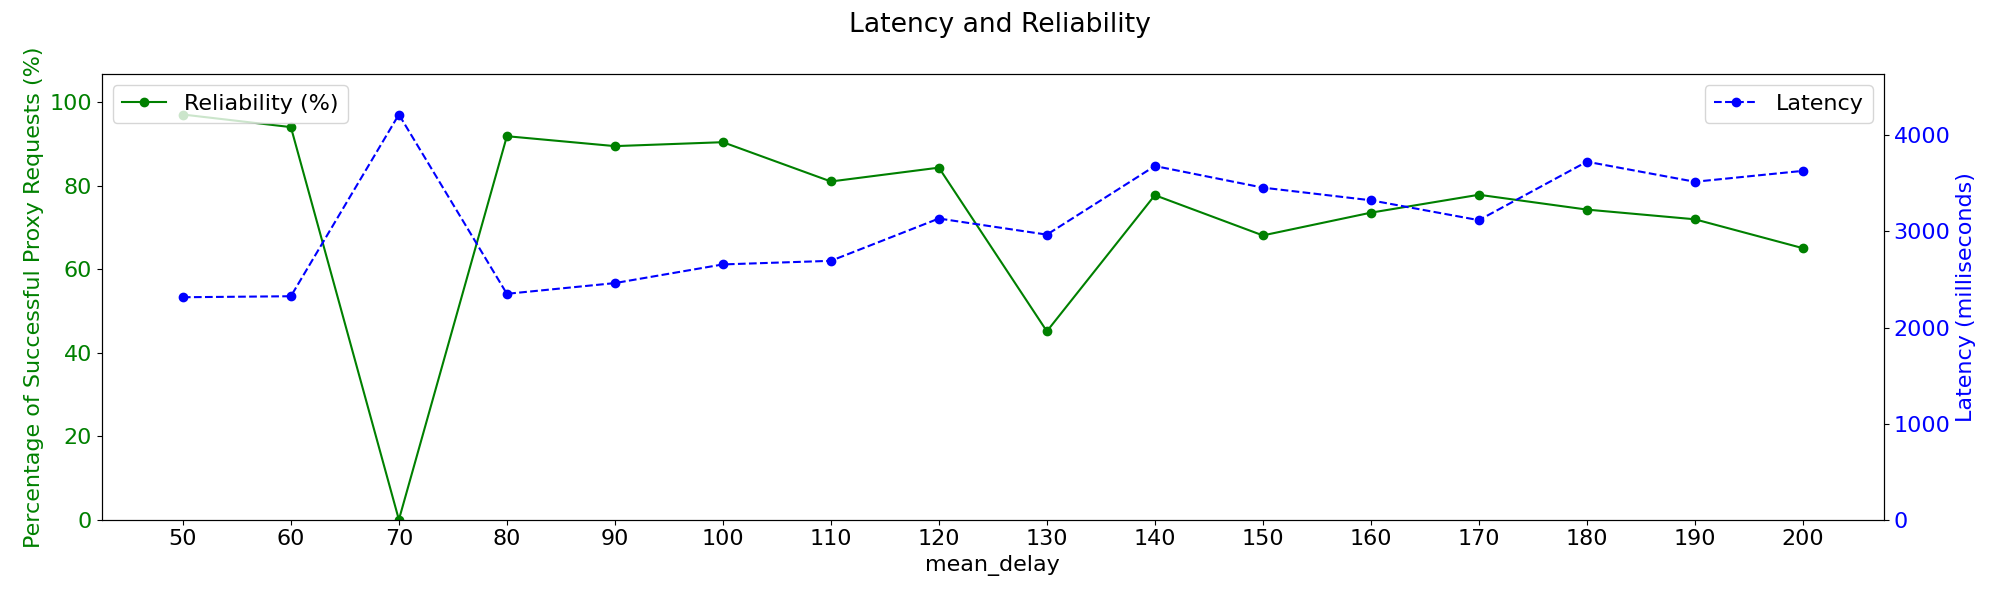
\includegraphics[width=\textwidth]{plots/delays_reliability_latency.png}
        \caption{}
        \label{fig:heatmap_bandwidth.png}
    \end{subfigure}
\end{figure}


In \textbf{autoref}, max retreive value over 9 and below 3 increases the latency. We believe below three it is not enough to send the full web page information from the web proxy, and over 9, there is an added overhead for the provider and client to process all the dummy messages which increases latency. As mentioned in \textbf{autoref}, these experiments were run with \textbf{url} proxy requests, and rnuning this experiment with a wider variety of websites would be beneficial. However to accomodate larger websites with multiple body messages from the web proxy, we choose the max retreieve \textbf{X} going forward.

For time pull it is no surprise that lower time pull decreases latency and increases bandwidth.
essentially, we believe that as we are tuning our system to browse the internet, we do not need to have a very big max retrieve value but the time pull should be low.


\textbf{TODO: add plot that shows max retreive average latency over time pulls}

\textbf{Talk about how we believe removing/replacing the providers would be beneficial and not retract from the anonymity}
In \textbf{autoref} section, it is mentioned that providers do not serve their main purpose of providing sender receiver online unobservibility. If loopix integration into fledger is only to be used for web proxy module, it might be beneficial to replace providers with simple entry nodes that will not store message but directory send the traffic to the client. \textbf{The client needs to know the network anyway, so they're kinda useless here} Mixnodes in the first and final layers of mix network could be used for this purpose, and would significantly reduce end-to-end latency while not affecting privacy properties. However, if fledger loopix module would be used for other purposes such as private messaging, providers could still provide better privacy than not. We leave this extension/study of fledger loopix module to future work.

%-------------------
\subsection{Scalability}
Although we were not able to set up a experiments with larger number of nodes, in this section we try to demonstrate that this integration of Loopix Anonymity System into Fledger is scalable to many more nodes in the network. The same way we changed the cover traffic volume to accomodate the change in payload values and mean delay to keep the \textbf{mean number of messages at a mixnode} the same, we can adjust cover traffic to accomodate changing number of mixnodes and clients.

\textbf{insert graphs}
Here we show, path length two, 2 clients, 5 and 10 clients each with the same latency and incoming messages, but adjusted volume of cover traffic. As long as the providers can accomodate the incoming messages from many clients, loopix integraion into fledger is scalable. \textbf{as mentioned in autoref, ideally we would get rid of providers all together.}

%-------------------
\section{Reliability Mechanisms}
%-------------------
In section this section, each measurement is taken within a simulation of 980 seconds  (\(\approx 16\) minutes). The nodes are again allowed get started for 15 seconds, after which Fledger Loopix module is started. After about 5 minutes of normal operations, one of the mix nodes at layer one is stopped, after another 5 minutes one of the mixnodes at the second layer stopped, and finally after another 5 minutes, one of the mixnodes at the final layer of the mix network is stopped. The simulation continues to run for another 5 minutes with only one node at each layer, with the clients being unaware that the mixnodes are dead. 

\textbf{maybe insert a figure here}

Here the web proxy timeout is set to 6 seconds, approximately 2-3 times the average latency with this configuration. The timeout is set to this value to be able to study the effectiveness of the mechanisms in this section.
%-------------------
\subsection{Retrying}

%-------------------
\subsection{Duplicate Messages}

%-------------------
\subsection{Combination of Retrying and Duplicate Messages}

\subsection{Raptor Code}
\textbf{I don't think I'll have time to implement this}

%%%%%%%%%%%%%%%%%%%%%%
\chapter{Related Work}
%%%%%%%%%%%%%%%%%%%%%%

% The related work section covers closely related work. Here you can highlight
% the related work, how it solved the problem, and why it solved a different
% problem. Do not play down the importance of related work, all of these
% systems have been published and evaluated! Say what is different and how
% you overcome some of the weaknesses of related work by discussing the 
% trade-offs. Stay positive!

% This section is usually 3-5 pages.

\textbf{I will probably skip this because of sections \autoref{sec:mixers} and \autoref{sec:reliable_message_delivery}}

%%%%%%%%%%%%%%%%%%%%
\chapter{Conclusion}
%%%%%%%%%%%%%%%%%%%%

% In the conclusion you repeat the main result and finalize the discussion of
% your project. Mention the core results and why as well as how your system
% advances the status quo.

\cleardoublepage
\phantomsection
\addcontentsline{toc}{chapter}{Bibliography}
\printbibliography

% Appendices are optional
% \appendix
% %%%%%%%%%%%%%%%%%%%%%%%%%%%%%%%%%%%%%%
% \chapter{How to make a transmogrifier}
% %%%%%%%%%%%%%%%%%%%%%%%%%%%%%%%%%%%%%%
%
% In case you ever need an (optional) appendix.
%
% You need the following items:
% \begin{itemize}
% \item A box
% \item Crayons
% \item A self-aware 5-year old
% \end{itemize}

\end{document}